\subsection{Work in Progress}

\subsubsection{Merge Translation and Shelf Linearization}

A common Git use case are modifications performed by multiple users in their local branches and then merged all together into the main development branch of the remote repository. 
For this scenario every user's branch becomes a shelf (see "Shelf Branches" section). Subversion users are not accustomed to
to this kind of workflow and would prefer to see linear history of changes on the main branch, where each revision have been committed by a particular user.
\\\\
As an experimental feature for that use case, we introduce a shelf linearization approach shown at the diagram \ref{boat_merge_keep_history_linear_git_to_svn}.
\begin{center}
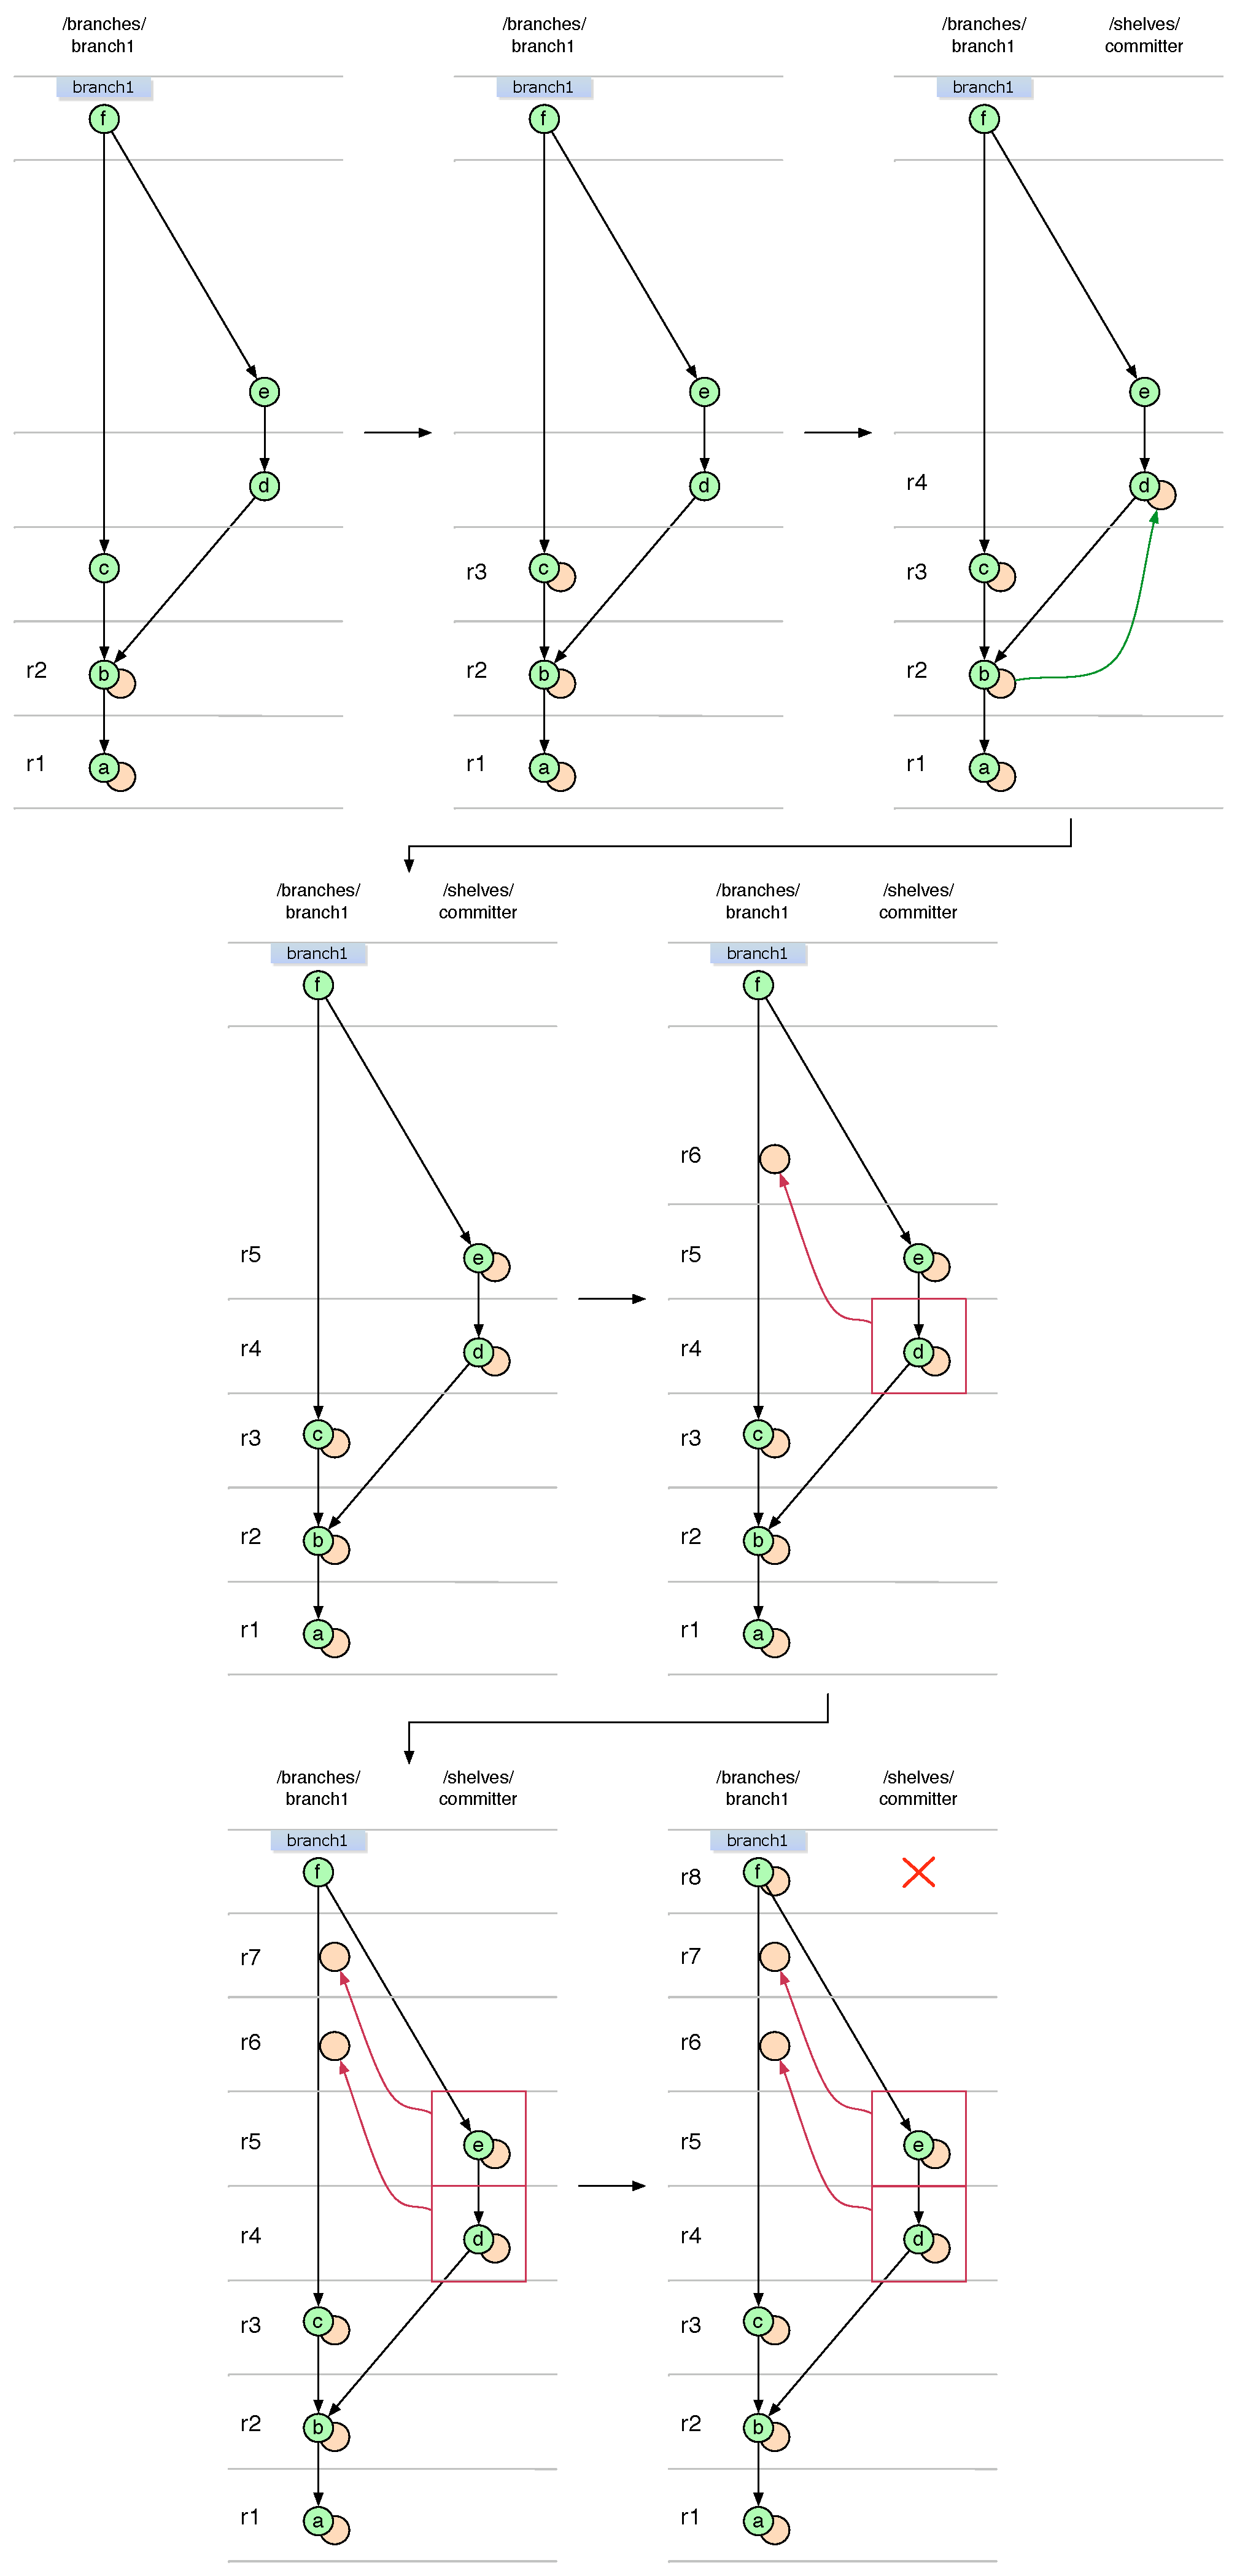
\includegraphics[height=18.9cm]{img/diagrams/boat_merge_keep_history_linear_git_to_svn.pdf}%
\captionof{figure}{Merge of Git branch which is available from another branch being translated to a sequence of Subversion revisions.}
\label{boat_merge_keep_history_linear_git_to_svn}%
\end{center}

If commit \emph{c} and a pair of commits \emph{d} and \emph{c} affects independent sets of files, 
then it is possible to imitate linear history for branch \emph{branch1}. 
For that purpose Translator creates three revisions r6, r7, r8 instead of a single revision that would be mapped to merge commit \emph{f}.
\\\\
For every commit at shelf Translator generates a revision with synthetic cherry-pick merge of the revision mapped to this commit. Finally revision r8 is the revision corresponding to commit \emph{f} and also it has the history of the shelf within svn:mergeinfo property. Hence mapping commit \emph{f} to revision r8 is valid. Having these revisions at branch branch1 Subversion users see history of branch branch1 linear.
\\\\
Shelf linearization has a few drawbacks:
\begin{enumerate}
\compactlist
	\item Main branch and shelf must not modify the same file, otherwise the approach is not applicable.
	\item At revisions r7 and r8 there could appear build failures since at this revision branch1 state is generated by Translator with no additional checks.
	\item This approach violates commits to revision mapping, since \emph{f} commit should be mapped to a sequence of revision r6, r7 and r8 instead of one single revision. It needs an extension of suggested commit to revision mapping.
\end{enumerate}

Shelf linearization could be applied to any branch to keep history linear, but \emph{shelf} branch is the most common target
for the linearization approach.

\subsubsection{Git Forks}

Git Fork is an unique feature of GitHub. First version of Translator translates Git Fork and pull request using Subversion concepts of copy and merge,
but makes not attempt to represent Subversion operations as a Git Fork.\\\\
Further versions of Translator might extend translation
rules so that some specific copies and merges performed in Subversion repository are translated into Git Fork.

\subsubsection{Fork-aware Subversion Repository Layout}

In order to support translation of Git Forks to Subversion repository in the most efficient way, 
preserving history of original repository in the forked one and allowing further translation of
Git pull requests in terms of Subversion merges, 
Subversion repository layout must have the following structure:\\

/\emph{user}/trunk\\
/\emph{user}/branches\\
/\emph{user}/tags\\

where \emph{user} is name of the user who have created this repository or 
corresponding Git repository. Each Git fork will add the following directories to the above:\\

/\emph{fork-user}/trunk\\
/\emph{fork-user}/branches\\
/\emph{fork-user}/tags\\

where \emph{fork-user} is the name of the user who have forked original Git repository or fork of the original Git repository.
\\\\
In order to identify uniquely Subversion repository backend, both user name and name of the project are needed. Thus,
Subversion users will use the following URLs to access Subversion repository:\\

\textbf{Project Trunk Location}: http://svnhub.com/\emph{project}/\emph{user}/trunk\\
\textbf{Repository Root}: http://svnhub.com/\emph{project}\\

Last URL doesn't allow to identify Subversion repository as it is shared by the independent projects of the same 
name created by different users. In order to resolve this ambigousity it will be necessary to require user authorization
on access to repository root URL. In general, repository root does not need to be access in the course of normal
Subversion workflow, but certain versions of Subversion client does access it due to the bugs in implementation and this 
should be taken into account by Translator.\\\\
Other schemes for Subversion repository layout and access URLs might be proposed. For instance, \emph{project} component
might be moved to the host name, so that project trunk URL will look like: http://\emph{project}.svnhub.com/\emph{user}/trunk
\\\\
Exact scheme will be defined in the future versions of this specification in case effective Git Forks translation support 
is required.
\subsubsection{Forked Repository}
Git Repository Fork creates new Git repository on GitHub. This new forked Git repository has the following 
important features:
\begin{itemize}
\item Repository is assigned to a particular \emph{user}
\item Repository holds information on its \emph{origin} and includes complete origin history
\item Changes made in the forked repository might be \emph{pulled back} into origin repository
\end{itemize}

These features make its natural to translate Git Fork into a copy \emph{within} Subversion repository. Single fork 
operation is translated into a revision which copies Subversion repository top-level directories into another top-level directory. 
Thus, fork performed by the \emph{user} will be translated into the following revision:\\

rN user\\ 
=======================\\
Fork comment             \\
=======================\\
A /\emph{fork-user}/trunk copied from /\emph{user}/trunk at rM\\
A /\emph{fork-user}/branches copied from /\emph{user}/branches at rM\\
A /\emph{fork-user}/tags copied from /\emph{user}/tags at rM\\

Repository layout after the fork:\\

/\emph{user}/trunk\\
/\emph{user}/branches\\
/\emph{user}/tags\\
/\emph{fork-user}/trunk\\
/\emph{fork-user}/branches\\
/\emph{fork-user}/tags\\\\
Changes made by Subversion users to the files and directories in /\emph{fork-user} directory are translated to the Git commits in the forked Git
repository and vice versa - Git commits in the forked Git repository are translated into Subversion revisions which modifies files
and directories in the corresponding /\emph{fork-user} directory of Subversion repository.

\subsubsection{Pull Request}

Accepted Git pull request is represented as a Git commit(s) in the original Git repository. Those Git commits are translated into Subversion
revision using standard translation rules. Additionally, Translator updates merge tracking information on the affected branches, so that
from the Subversion user perspective, translated revision looks like a merge of changes from the corresponding branches in the /\emph{user} directory. 
Merge tracking information in Subversion repository after translation may look like:\\

/\emph{user}/trunk : from /\emph{fork-user}/trunk:10-11\\
/\emph{user}/branches/b : from /\emph{fork-user}/branches/b:10-11\\

assuming that revisions 10 and 11 represent changes in the forked Git repository.

\subsection{Concepts not covered by this Specification}
This version of Translator specification does not cover translation of the following concepts:
\begin{itemize}
\item Subversion svn:keywords special property
\item Regular Subversion properties and Git attributes
\item Subversion revision properties and Git notes
\item Subversion svn:external property which uses HEAD revision
\item Subversion path based authentication
\end{itemize}

First version of Translator ignores above mentioned entities on translation and will do no attempt to translate them.